Trong Hình 7, các tiếp tuyến với các đường cong này đã được vẽ tại một số điểm. Ở phần (a), đường cong nằm phía trên các tiếp tuyến và $f$ được gọi là \textit{lõm lên} (\textit{concave upward}) trên $(a, b)$. Ở phần (b), đường cong nằm phía dưới các tiếp tuyến và $g$ được gọi là \textit{lõm xuống} (\textit{concave downward}) trên $(a, b)$.

\vspace{0.2cm}
\begin{center}
  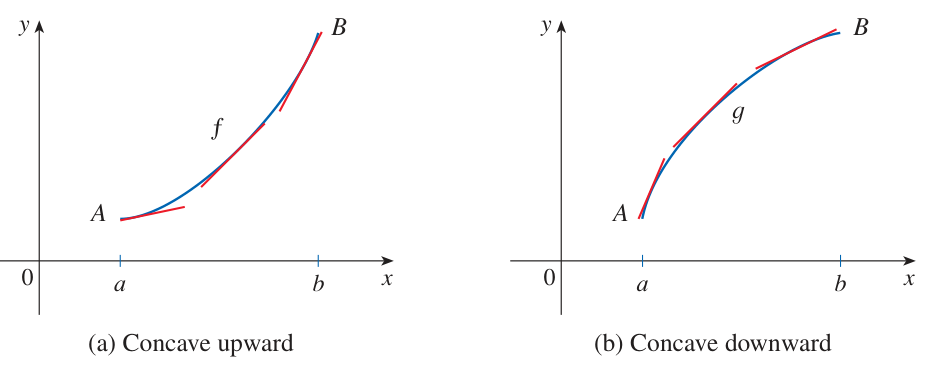
\includegraphics[width=0.98\linewidth]{images/p0335_fig1.png}
\end{center}
\vspace{-0.6cm}
\marginnote{\textsf{\textbf{HÌNH 7}}}[-0.5cm]

\vspace{0.3cm}
\marginnote{%
  \textbf{\textsf{Ký hiệu}}\\[2pt]
  {\small Ta dùng chữ viết tắt CU cho lõm lên (concave upward) và CD cho lõm xuống (concave downward).}
}[0.1cm]
\begin{tcolorbox}[colback=white, colframe=stewartred, boxrule=0.8pt, arc=0mm, left=8pt, right=8pt, top=6pt, bottom=6pt]
  {\color{stewartred}\textbf{Định nghĩa}}\quad Nếu đồ thị của $f$ nằm phía trên tất cả các tiếp tuyến của nó trên một khoảng $I$, thì $f$ được gọi là \textbf{lõm lên} trên $I$. Nếu đồ thị của $f$ nằm phía dưới tất cả các tiếp tuyến của nó trên $I$, thì $f$ được gọi là \textbf{lõm xuống} trên $I$.
\end{tcolorbox}

\vspace{0.2cm}
Hình 8 cho thấy đồ thị của một hàm số lõm lên (CU) trên các khoảng $(b, c)$, $(d, e)$, và $(e, p)$ và lõm xuống (CD) trên các khoảng $(a, b)$, $(c, d)$, và $(p, q)$.

\vspace{0.2cm}
\begin{center}
  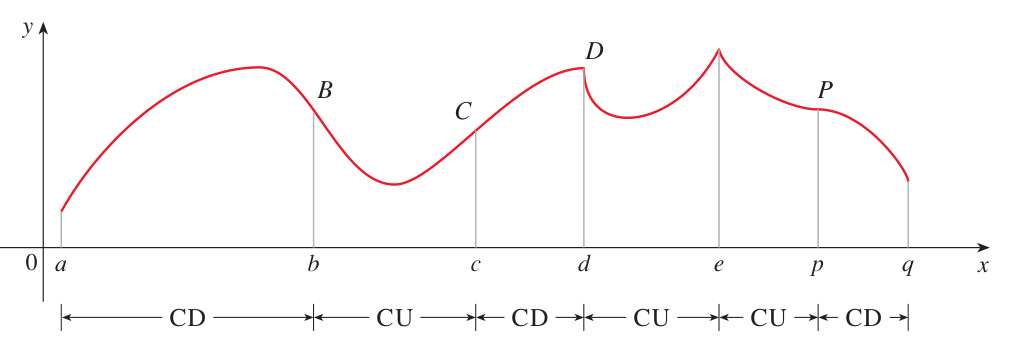
\includegraphics[width=0.98\linewidth]{images/p0335_fig2.png}
\end{center}
\vspace{-0.6cm}
\marginnote{\textsf{\textbf{HÌNH 8}}}[-0.5cm]

\vspace{0.3cm}
Hãy xem đạo hàm cấp hai giúp xác định các khoảng lồi lõm như thế nào. Quan sát Hình 7(a), bạn có thể thấy rằng, đi từ trái sang phải, hệ số góc của tiếp tuyến tăng dần. Điều này có nghĩa là đạo hàm $f'$ là một hàm tăng và do đó đạo hàm của nó $f''$ mang giá trị dương. Tương tự, trong Hình 7(b), hệ số góc của tiếp tuyến giảm dần từ trái sang phải, do đó $f'$ giảm và vì thế $f''$ mang giá trị âm. Lập luận này có thể đảo ngược và gợi ý rằng định lý sau đây là đúng. Một chứng minh được trình bày trong Phụ lục F với sự trợ giúp của Định lý Giá trị Trung bình.

\vspace{0.3cm}
\begin{tcolorbox}[colback=white, colframe=stewartred, boxrule=0.8pt, arc=0mm, left=8pt, right=8pt, top=6pt, bottom=6pt]
  {\color{stewartred}\textbf{Tiêu chuẩn xét tính lồi lõm}}\\[4pt]
  \textbf{(a)}\enspace Nếu $f''(x) > 0$ trên một khoảng $I$, thì đồ thị của $f$ lõm lên trên $I$.\\[3pt]
  \textbf{(b)}\enspace Nếu $f''(x) < 0$ trên một khoảng $I$, thì đồ thị của $f$ lõm xuống trên $I$.
\end{tcolorbox}
